\documentclass[11pt]{article}

%%%%%%%%%%%%%%%%%%%%%%%%%%%%%%%%%%%%%%%%%%%%%%%%%%%%
% Preamble:
%%%%%%%%%%%%%%%%%%%%%%%%%%%%%%%%%%%%%%%%%%%%%%%%%%%%
% Typical Packages:
\usepackage[utf8]{inputenc}
\usepackage{fullpage}
\usepackage{amsfonts}
\usepackage{amsmath}
\usepackage{amsthm}
\usepackage{amssymb}
\usepackage{mathrsfs}
\usepackage{graphicx}
\usepackage{color}
\usepackage{palatino}
\usepackage{url}
\usepackage{multicol}
\usepackage{enumerate}
\usepackage{ulem}
\usepackage{tikz}
\usepackage{tipa} 
\usepackage{upgreek}
\usepackage{hyperref}
\usepackage{verbatim}
\usepackage{caption}
\usepackage{fancyhdr}

\thispagestyle{empty}

% Title
\title{First Latex Project}
\author{Brooks Emerick}
\date{\today}

%%%%%%%%%%%%%%%%%%%%%%%%%%%%%%%%%%%%%%%%%%%%%%%%%%%%
% Start Document:
%%%%%%%%%%%%%%%%%%%%%%%%%%%%%%%%%%%%%%%%%%%%%%%%%%%%
\begin{document}

\maketitle


\section{First Section}


\begin{figure}[h]

\centering
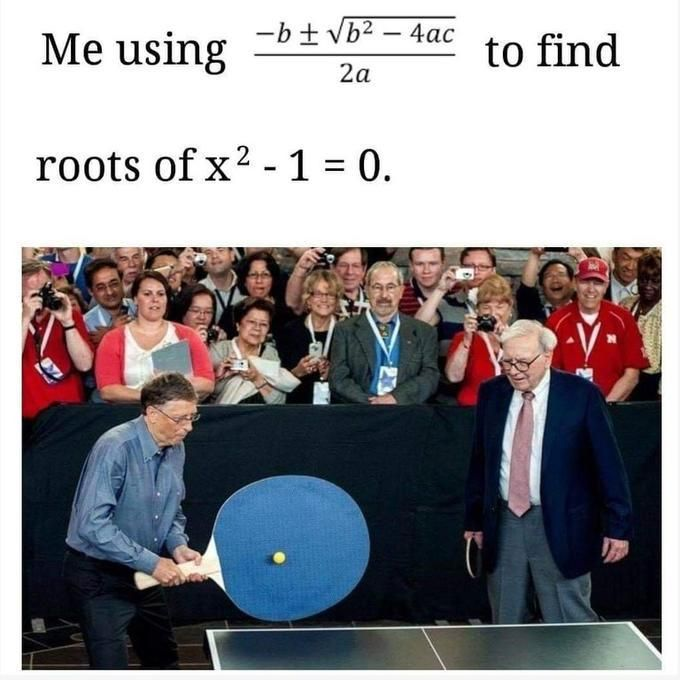
\includegraphics[width = .45\textwidth]{Figures/Histogram.jpeg}
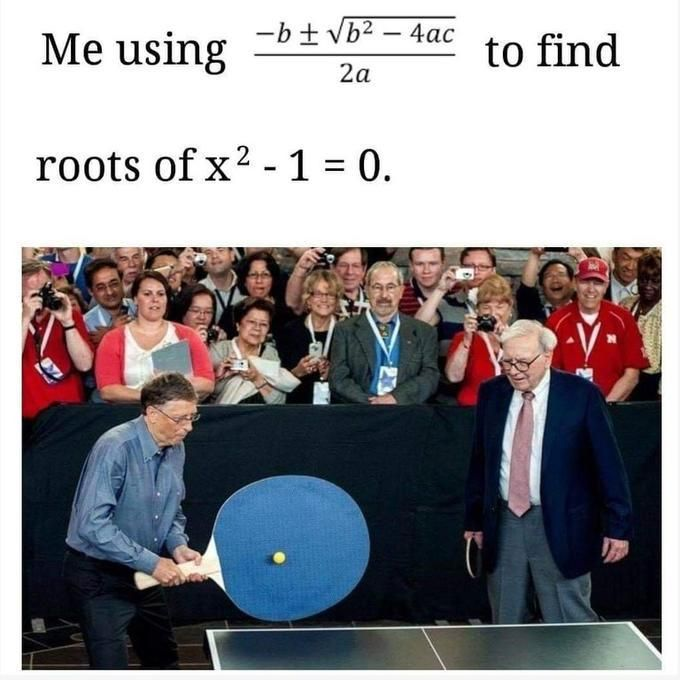
\includegraphics[width = .45\textwidth]{Figures/Histogram.jpeg}
\caption{This is Bill Gates with a giant ping pong paddle. }
\label{Bill}

\end{figure}


Remember the quadratic formula (e.g.~Figure \ref{Bill})















\end{document}